\subsection{Columnar}

\begin{frame}
    \frametitle{Columnar - Repaso}
    
    \begin{columns}
        \begin{column}{0.64\textwidth}
            Las bases de datos orientadas a columnas almacenan datos verticalmente por columnas en lugar de horizontalmente por filas, permitiendo un acceso más eficiente a datos específicos.
        \end{column}
        \begin{column}{0.34\textwidth}
            \centering
            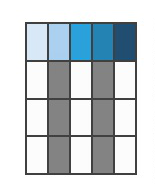
\includegraphics[width=0.7\textwidth]{images/Columnar.png}
        \end{column}
    \end{columns}

     
    
    Algunas de sus ventajas:

     
    
    \begin{itemize}
        \item  Mayor eficiencia en consultas sobre columnas específicas.  
        \item  Convenientes para análisis de grandes volúmenes de datos.  
        \item  Adecuadas para aplicaciones de business intelligence y análisis predictivo.
    \end{itemize}
    
\end{frame}

\begin{frame}
    \frametitle{Columnar - Ejemplos}
    Algunos ejemplos de bases de datos columnares son: 
    
    \begin{itemize}
        \item \textbf{Apache Cassandra}
        
        \item \textbf{Apache HBase}
        
        \item \textbf{ClickHouse}
    \end{itemize}

     
    
    Nos vamos a centrar en Apache HBase.
\end{frame}

\subsubsection{Apache HBase}

\begin{frame}
    \frametitle{Columnar - Apache HBase}
    \centering
    
\includegraphics[width=0.4\textwidth]{images/hbase-logo.png}
    \begin{itemize}
        \item Base de datos distribuida y escalable.  
        \item Desarrollada por la Apache Software Foundation.  
        \item Modelo de datos basado en tablas y columnas flexibles.  
        \item Almacenamiento de datos en archivos HFile en Hadoop HDFS.  
        \item Utiliza partición distribuida y replicación para alta disponibilidad.  
        \item Ofrece diferentes niveles de consistencia.
    \end{itemize}

\end{frame}


\begin{frame}{Operaciones Básicas en Hbase}

HBase proporciona un conjunto de comandos específicos que se utilizan para realizar diversas operaciones administrativas y de consulta.
      

    Algunos ejemplos son:

      
    \begin{enumerate}
        \item \textbf{create}: Crear una nueva tabla.  
        \item \textbf{put}: Insertar un valor en una celda de datos.  
        \item \textbf{get}: Recuperar datos de una fila.  
        \item \textbf{delete}: Eliminar una celda de datos.  
        \item \textbf{drop}: Eliminar una tabla.
    \end{enumerate}

\end{frame}

\begin{frame}[fragile]
\frametitle{Ejemplo de Uso}
\begin{verbatim}
hbase(main):001:0> create 'usuarios', 
                    'datos_personales', 'datos_contacto'
0 fila(s) en 1.2340 segundos
\end{verbatim}

\end{frame}

\begin{frame}[fragile]
\frametitle{Ejemplo de Uso}
\begin{verbatim}

hbase(main):002:0> put 'usuarios', '1001', 
'datos_personales:nombre', 'Juan'
0 fila(s) en 0.0510 segundos

hbase(main):003:0> put 'usuarios', '1001', 
'datos_personales:apellido', 'Pérez'
0 fila(s) en 0.0110 segundos

hbase(main):004:0> put 'usuarios', '1001', 
'datos_contacto:email', 'juan@example.com'
0 fila(s) en 0.0090 segundos
\end{verbatim}

\end{frame}

\begin{frame}[fragile]
\frametitle{Ejemplo de Uso}
\begin{verbatim}
hbase(main):005:0> get 'usuarios', '1001', 
{COLUMN => 'datos_personales'}
COLUMN                          CELL
 datos_personales:nombre        valor=Juan
 datos_personales:apellido      valor=Pérez
1 fila(s) en 0.0190 segundos
\end{verbatim}
\end{frame}

\begin{frame}[fragile]
\frametitle{Ejemplo de Uso}
\begin{verbatim}

hbase(main):006:0> delete 'usuarios', '1001', 
'datos_contacto:email'
0 fila(s) en 0.0230 segundos
\end{verbatim}
  
\begin{verbatim}
hbase(main):007:0> get 'usuarios', '1001'
COLUMN                          CELL
 datos_personales:nombre        valor=Juan
 datos_personales:apellido      valor=Pérez
1 fila(s) en 0.0190 segundos
\end{verbatim}

\end{frame}

\begin{frame}{Operaciones Avanzadas en HBase}
    \begin{enumerate}
        \item Escaneo de Rango  
        \item Filtros de Columnas y Filas  
        \item Transacciones y Consistencia  
        \item Replicación de Datos  
        \item Optimización de Rendimiento  
        \item Seguridad
    \end{enumerate}
\end{frame}